% LaTeX source for ``การเรียนรู้ของเครื่องสำหรับเคมีควอนตัม (Machine Learning for Quantum Chemistry)''
% Copyright (c) 2022 รังสิมันต์ เกษแก้ว (Rangsiman Ketkaew).

% License: Creative Commons Attribution-NonCommercial-NoDerivatives 4.0 International (CC BY-NC-ND 4.0)
% https://creativecommons.org/licenses/by-nc-nd/4.0/

\chapter{การทำนายคุณสมบัติของโมเลกุล}
\label{ch:predict_molprop}

%--------------------------
\section{แนวทางการปฏิบัติ}
%--------------------------

แนวทางปฏิบัติ (Best Practice) หรือลำดับขั้นตอนสำหรับการนำ ML มาประยุกต์กับเคมีควอนตัมสามารถแบ่งออกเป็น 6 ขั้นตอนง่าย ๆ ได้ดังนี้
\idxen{Best Practice}

\begin{enumerate}
    \item ทำความสะอาดข้อมูลดิบ (Raw Data Cleaning)
    \item เลือก Representation/Descriptor ที่จะนำมาคำนวณ Feature 
    \item เลือกอัลกอริทึม ML ที่เหมาะสมกับโจทย์ของเรา 
    \item ฝึกสอนโมเดลและทำนายคำตอบ
    \item ศึกษาผลกระทบจากการเปลี่ยน Hyperparameter และทำ Validation
    \item ประเมินประสิทธิภาพของโมเดลและวิเคราะห์ผลการทำนาย
\end{enumerate}

ขั้นตอนแรกสุดเลยก็คือเป็นการเตรียมข้อมูลดิบนั่นก็คือข้อมูลทางเคมีเบื้องต้นที่เรามี โดยส่วนใหญ่แล้วนักเคมีเชิงคำนวณมักจะเริ่มต้นด้วยข้อมูลพิกัด%
คาร์ทีเซียน (Cartesian Coordinates) ของชุดโมเลกุลที่ต้องการศึกษา เช่น โมเลกุลอินทรีย์ ลำดับถัดมาคือเราจะต้องเลือก Representation 
ที่เราต้องการนำมาคำนวณมาคุณสมบัติต่าง ๆ ของโมเลกุล ซึ่งเรามักจะได้มาจากการคำนวณด้วยวิธีแบบดั้งเดิม โดยการคำนวณ Representation 
นั้นก็จะมีให้เลือกมากมาย ขึ้นอยู่กับความสอดคล้องของอินพุต (Feature ที่เราคำนวณ) กับเอาต์พุตที่เราต้องการจะทำนาย ซึ่งขั้นตอนนี้จะเป็นการ%
สร้างชุดข้อมูลนั่นเอง เมื่อเราได้ชุดข้อมูลแล้ว เราอาจจะมีขั้นตอนที่แทรกเข้ามาเพื่อช่วยให้เราเข้าใจชุดข้อมูลได้มากขึ้น เช่น เราอาจจะใช้สถิติเข้ามา%
ช่วยคำนวณค่าทางสถิติของชุดข้อมูลก่อนนำไปฝึกสอนโมเดล เช่น คำนวณค่ากลางหรือพารามิเตอร์ที่ให้เราเข้าใจการกระจายตัวในชุดข้อมูลรวมไปถึง%
ความสำคัญ (Importance) ของ Feature แต่ละตัวในชุดข้อมูล การทำแบบนี้จะช่วยให้เราเข้าใจว่า Feature ตัวไหนที่ \enquote{น่าจะ} มีผล%
ต่อประสิทธิภาพของโมเดลเรามากที่สุด เมื่อเราได้ชุดข้อมูลที่มีความเหมาะสมแล้ว ขั้นตอนต่อมาคือการเลือกเทคนิคหรืออัลกอริทึมของ ML ที่เราต้องการ%
จะใช้ เริ่มต้นเราอาจจะยังไม่ต้องไปใช้เทคนิคที่อลังการมากก็ได้ ซึ่งการเลือกใช้เทคนิคง่าย ๆ เช่น Ridge Regression ก็อาจจะทำให้เรามีโมเดล MLP
ที่มีประสิทธิภาพมาก ๆ แล้วก็ได้ เพราะการที่เราไปใช้เทคนิคที่ซับซ้อนตั้งแต่แรกนั้น มันอาจจะไม่ได้การันตีว่าเราจะได้โมเดลที่ดีเสมอไป และนอกจากนี้%
ยังเสียเวลาอีกด้วย ตัวอย่างเช่น ผู้เขียนมักจะเห็นหลาย ๆ คนที่เริ่มฝึกสอนโมเดลด้วย Deep Neural Network โดยการใช้เทคนิคขั้นสูงกับข้อมูลที่%
มีความเรียบง่าย (ขี่ช้างจับตั๊กแตน) ซึ่งตรงจุดนี้บางครั้งมันก็มีความไม่เหมาะสมระหว่างเทคนิคและข้อมูลที่เรามี โดยตรงจุดนี้ก็ขึ้นอยู่กับวิจารณญาน%
ของแต่คนครับ เมื่อเราเลือกวิธี ML ได้แล้ว ขั้นตอนต่อมาก็คือการสร้างโมเดลและฝึกสอนกับ Training Set โดยในขั้นตอนนี้เราอาจจะลองสร้างหลาย ๆ 
โมเดลและทำการปรับ Hyperparameter ไปด้วยก็ได้ (ควรจะเปลี่ยนค่าอย่างเป็นระบบ ไม่ควรเปลี่ยนแบบมั่ว ๆ) นอกจากนี้เราอาจจะยังทำ Validation 
ด้วยก็ได้ เมื่อเราได้โมเดลที่ถูกฝึกสอนมาแล้ว ลำดับต่อมาก็คือการทำนายหรือพยากรณ์คำตอบนั่นเอง โดยเราจะต้องมาประเมินประสิทธิภาพของโมเดล%
ในขั้นตอนนี้ด้วย เราจะต้องมาวิเคราะห์ถึงปัจจัยที่ส่งผลต่อค่าที่เราได้ออกมา พยายามหาความเชื่อมโยงระหว่าง Feature, ML Algorithm และ%
พารามิเตอร์อื่น ๆ เมื่อเราได้โมเดลที่ถูกฝึกสอนมาอย่างดีและมีประสิทธิภาพที่อยู่ในเกณฑ์ที่ยอมรับได้แล้วนั้น เราก็จะมีโมเดลที่พร้อมจะไปใช้งานจริงครับ

\begin{figure}[H]
    \centering
    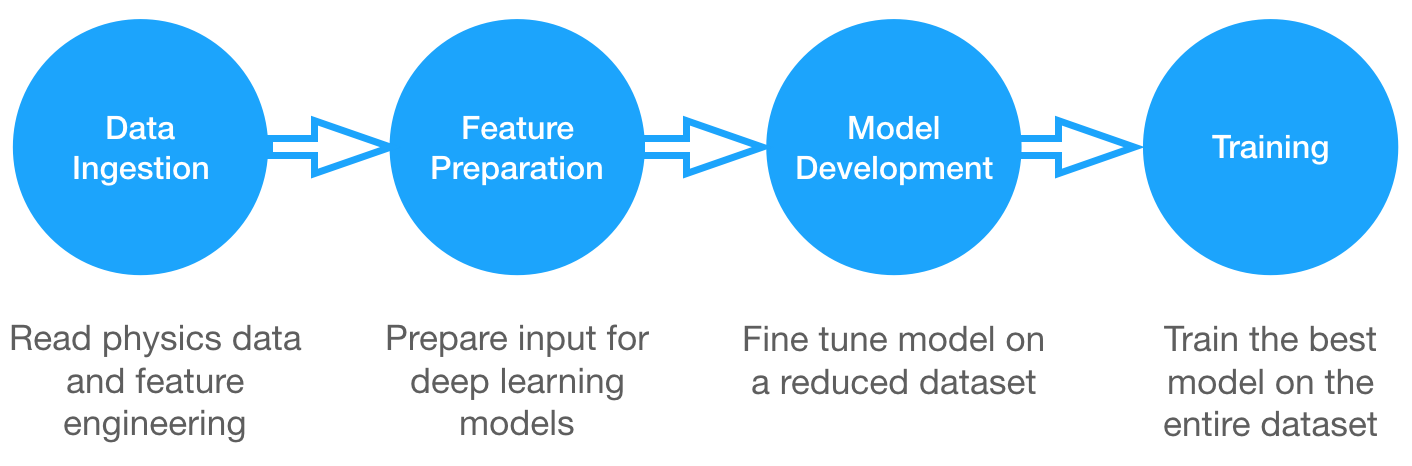
\includegraphics[width=\linewidth]{fig/ml_pipeline.png}
    \caption{แนวทางและขั้นตอนการสร้างโมเดลปัญญาประดิษฐ์ (เครดิตภาพ: https://vitalflux.com)}
    \label{fig:ml_pipeline}
\end{figure}

%--------------------------
\section{การเลือกโมเดลที่เหมาะสม}
%--------------------------

\begin{figure}[H]
    \centering
    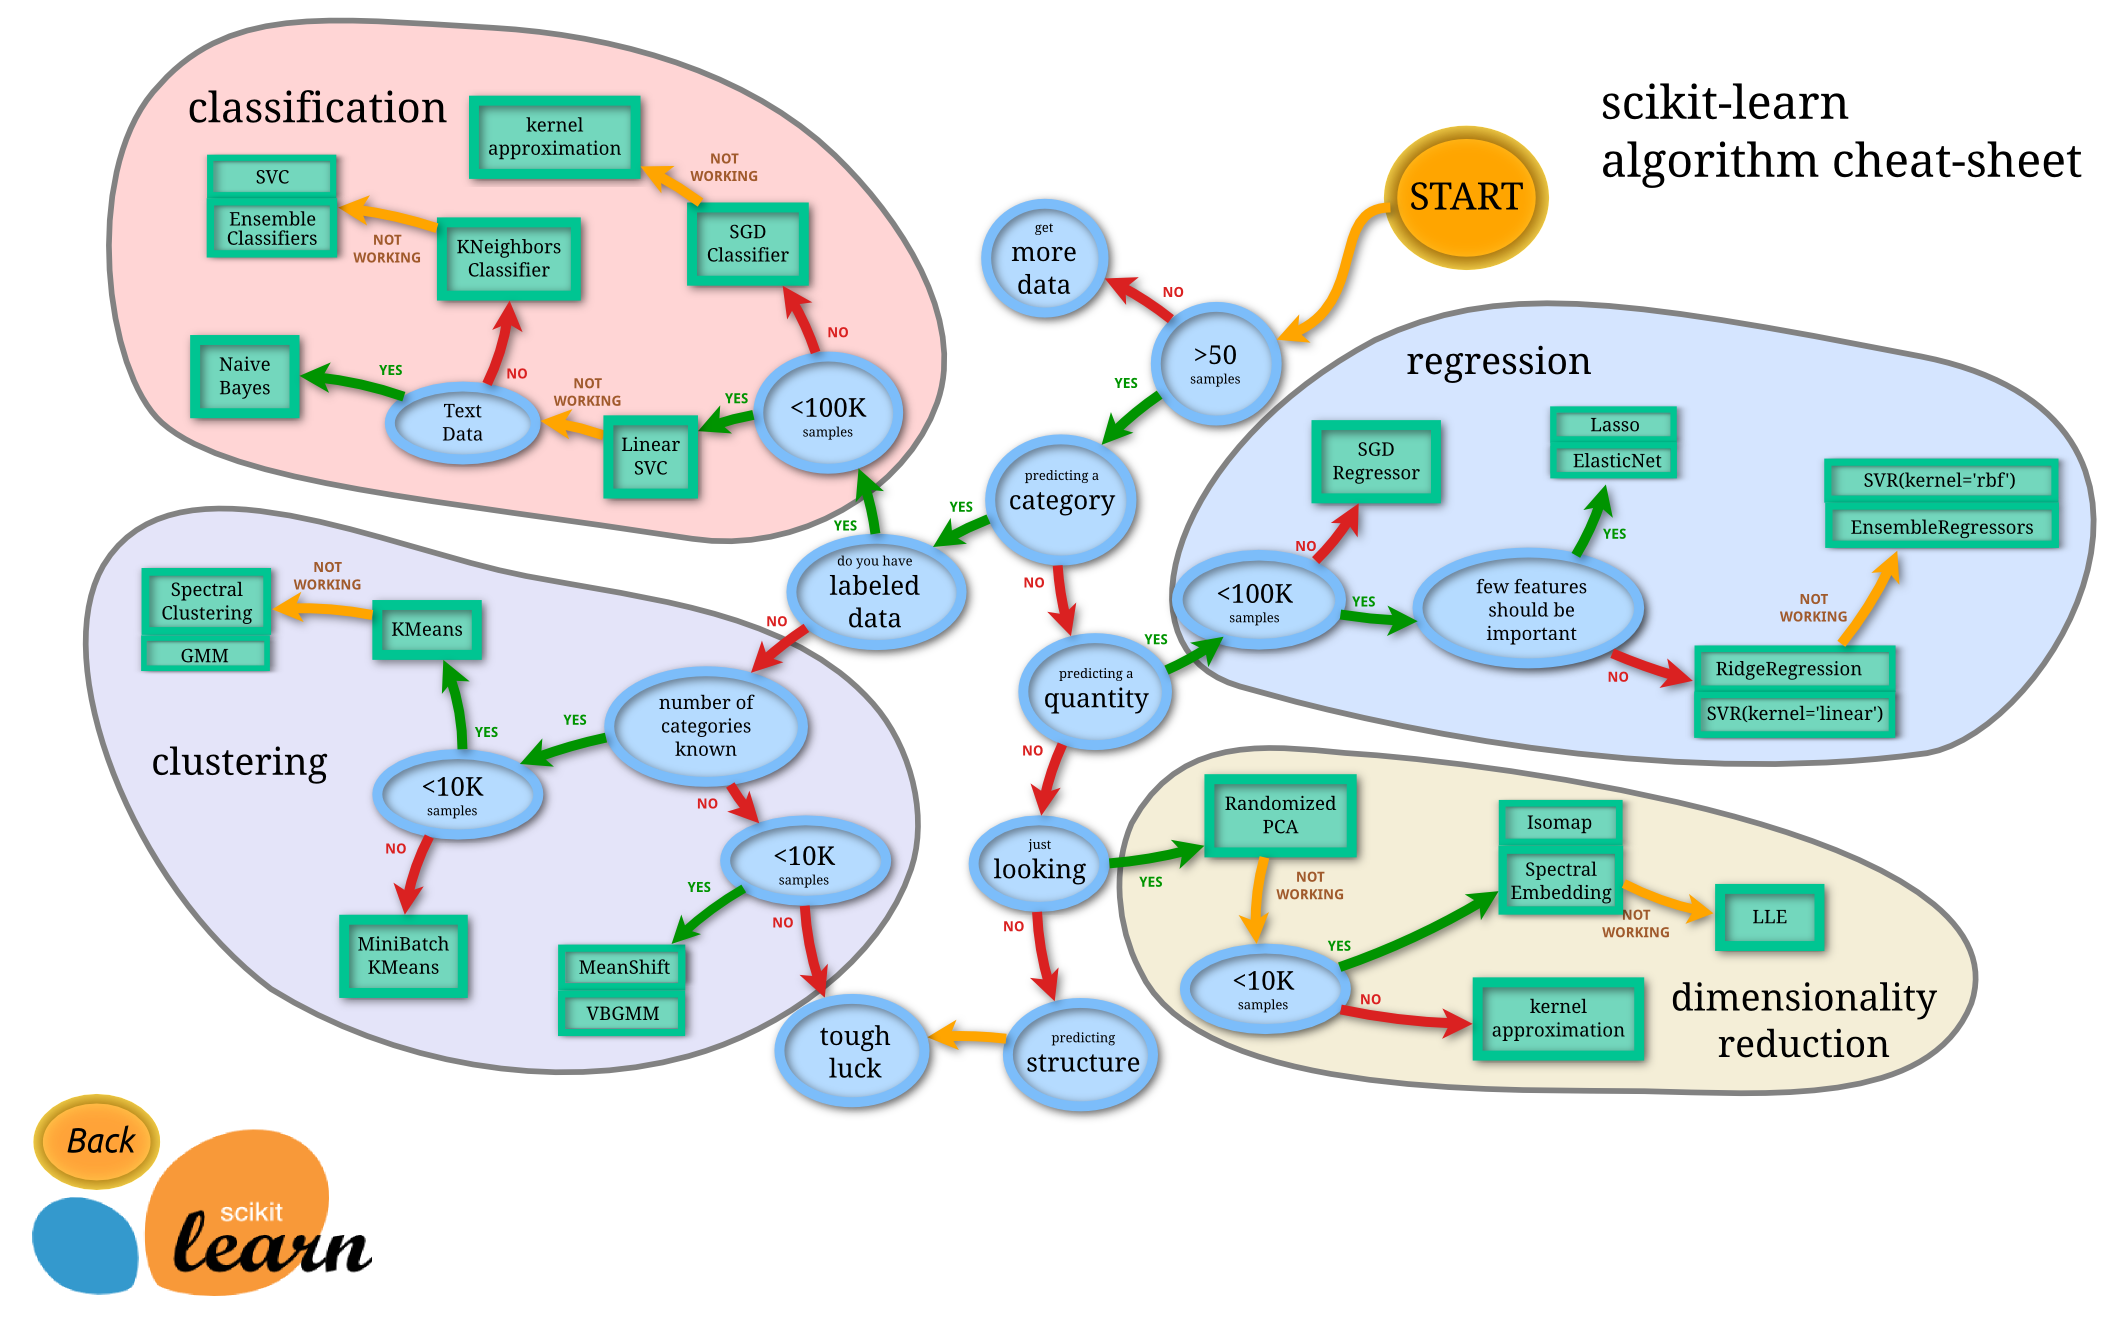
\includegraphics[width=1.3\linewidth,angle=90]{fig/ml_map.png}
    \caption{แผนภาพการเลือกใช้โมเดลปัญญาประดิษฐ์ (เครดิตภาพ: https://scikit-learn.org)}
    \label{fig:ml_map}
\end{figure}

\begin{itemize}
    \item Linear kernel : $K(x_i, x_j) = x_i \cdot x_j$
    \item Polynomial : $K(x_i, x_j; a, b) = (x_i \cdot x_j + a)^b$
    \item Gaussian kernel : $K(x_i, x_j; w, \sigma) = \mathrm{exp}\left(-\frac{|x_i-x_j|^2}{2\sigma^2}\right)$
    \item Laplacian kernel : $K(x_i, x_j; w, \gamma) = \mathrm{exp}\left(-{|x_i-x_j|}\right)$
\end{itemize}

%--------------------------
\section{การทำนายพลังงานรวมของโมเลกุล}
%--------------------------

%--------------------------
\section{การทำนายพื้นผิวพลังงานศักย์}
%--------------------------

การทำนายพื้นผิวพลังงานศักย์ (Potential Energy Surface หรือ PES)

Machine Learning Potentials (MLP) เป็นอีกหนึ่งเครื่องมือสำคัญสำหรับการจำลองในระดับอะตอม (Atomistic simulation) 
โดยเฉพาะการศึกษาพลังงานศักย์ของโมเลกุล\autocite{behler2016,botu2017,brockherde2017,deringer2019,noe2020} 
MLP แบ่งออกได้เป็นสองประเภทตามรูปแบบของอัลกอริทึมของ ML คือ Kernel-based Potentials กับ Neural Network-based Potentials

\begin{itemize}
    \item Gaussian Approximation Potentials (GAP)\autocite{bartok2010}
    \item Moment Tensor Potentials (MTP)\autocite{shapeev2016}
    \item Spectral Neighbor Analysis Potentials (SNAP)\autocite{thompson2015}
\end{itemize}


- High-dimensional Neural Network Potentials (HDNNP)\autocite{behler2007}
- ANAKIN-ME หรือเรียกสั้น ๆ ว่า ANI (ชื่อเต็มคือ (Accurate NeurAl networK engINe for Molecular Energies)
    - ANI-1x\autocite{smith2017}
    - ANI-1ccx\autocite{smith2018}
    - ANI-2x\autocite{smith2019}

%--------------------------
\section{การจำลอง Force Field}
%--------------------------

การทำนายหรือพยากรณ์แรง (Forces) และพลังงาน (Energies) ของโมเลกุลนั้นเรียกอีกอย่างหนึ่งว่าการสร้างโมเดล ML Force-field 
เริ่มต้นสมมติว่าเรามีชุดข้อมูลที่มี Feature Vector ซึ่งเขียนแทนด้วย $\mathbf{D}$ และมีอนุพันธ์แบบเวกเตอร์ (Divergence) เป็น 
$\nabla_{\mathbf{r_i}} \mathbf{D}$ และมีข้อมูลเพิ่มเติมคือพลังงาน $E$ และแรง $\mathbf{F}$ ของระบบ (โมเลกุล) สำหรับการฝึกสอน
เราจะสร้าง Neural Network (เขียนแทนด้วย $f$) เพื่อสร้างโมเดลสำหรับการทำนายพลังงาน ($\hat{E} = f(\mathbf{D})$)
\footnote{เครื่องหมาย $\hat{}$\, (อ่านว่า \enquote{hat}) ที่อยู่ด้านบนของตัวแปรเป็นส่งที่บ่งบอกว่าค่าที่เราจะทำนายของตัวแปรนั้น ๆ}
ซึ่งเราสามารถคำนวณแรงได้โดยตรงจากค่าติดลบของ Gradient ของพลังงานเทียบกับพิกัดตำแหน่งของอะตอมนั้น ๆ ดังนั้นแรงที่ได้จะเป็นปริมาณต่ออะตอม
ยกตัวอย่างเช่นแรงของอะตอม $i$ สามารถคำนวณได้จากสมการต่อไปนี้ (โดยใช้เวกเตอร์แบบแถว)
\idxen{Force Field}

\begin{align}\label{eq:force_pred}
\hat{\mathbf{F}}_i &= - \nabla_{\mathbf{r_i}} f(\mathbf{D}) \\
&= - \nabla_{\mathbf{D}} f \cdot \nabla_{\mathbf{r_i}} \mathbf{D}\\
&= - \begin{bmatrix}
    \frac{\partial f}{\partial D_1} & \frac{\partial f}{\partial D_2} & \dots
\end{bmatrix}
\begin{bmatrix}
    \frac{\partial D_1}{\partial x_i} & \frac{\partial D_1}{\partial y_i} & \frac{\partial D_1}{\partial z_i}\\
    \frac{\partial D_2}{\partial x_i} & \frac{\partial D_2}{\partial y_i} & \frac{\partial D_2}{\partial z_i}\\
    \vdots & \vdots & \vdots \\
\end{bmatrix}
\end{align}

จากสมการ \ref{eq:force_pred} นั้นเราอธิบายได้ว่า $\nabla_{\mathbf{D}} f$ เป็นค่าอนุพันธ์ของคำตอบของโมเดล ML ซึ่งจะเทียบกับ
Descriptor $\mathbf{D}$ และ $\nabla_{\mathbf{r_i}} \mathbf{D}$ เป็น อนุพันธ์ของ Descriptor ที่เทียบกับตำแหน่งของอะตอม
ซึ่งตามที่เราได้ศึกษามาก่อนหน้านี้ว่า Neural Network นั้นจะให้คำตอบที่เป็นแบบ Analytical Solution

%--------------------------
\section{การทำนายพลังงานกระตุ้นของปฏิกิริยาเคมี}
%--------------------------

พลังงานกระตุ้น (Activation Energy) เป็นค่าพลังงานที่บ่งบอกถึงความยากง่ายในการทำให้ปฏิริยาเคมีสามารถดำเนินไปได้ ณ สภาวะหนึ่ง ๆ

%--------------------------
\section{การทำนายประจุของอะตอม}
%--------------------------

%--------------------------
\section{การทำนายไดโพลโมเมนต์}
%--------------------------

%--------------------------
\section{การทำนายค่าคู่ควบเชิงเล็กอิเล็กทรอนิกส์}
%--------------------------

ค่าคู่ควบเชิงเล็กอิเล็กทรอนิกส์ (Electronic Coupling) คือค่าความเกี่ยวเนื่องเชิงอิเล็กทรอนิกส์ระหว่าง 2 สถานะใด ๆ เช่นสถานะเริ่มต้นและ%
สถานะสิ้นสุดในกระบวนการทางควอนตัม

- Electron transfer Coupling
- Nonadiabatic Coupling

%--------------------------
\section{การทำนายสเปกตรัม}
\idxth{การทำนายสเปกตรัม}
%--------------------------

การทำนายสเปกตรัมเป็นอีกหนึ่งหัวข้องานวิจัยทางด้านเคมีควอนตัมที่ได้รับความสนใจเป็นอย่างมากนั่นก็เพราะว่าเทคนิคทางสเปกโทรสโกปีนั้นมีประโยชน์%
อย่างมากในงานทางด้านเคมีสังเคราะห์ ทั้งเคมีอินทรีย์และเคมีอนินทรีย์ รวมไปถึงด้านอื่น ๆ เช่น วัสดุศาสตร์หรือพอลิเมอร์ด้วย 

เทคนิคสเปกโทรสโกปีเป็นเทคนิคที่เกี่ยวข้องกับแสงซึ่งเป็นคลื่นแม่เหล็กไฟฟ้าที่มีลักษณะเป็นแถบพลังงาน (Spectrum) โดยมีความยาวคลื่นตั้งแต่ในช่วง%
คลื่นวิทยุ คลื่นไมโครเวฟ คลื่นอินฟราเรด คลื่นในช่วงที่สายตามองเห็น รวมถึงคลื่นอัลตราไวโอเลต สำหรับคลื่นแม่เหล็กไฟฟ้าที่นักเคมีมักจะสนใจนั้นจะ%
เกี่ยวข้องโดยตรงกับการระบุถึงความจำเพาะเจาะจงของโมเลกุล นั่นคือคลื่นแม่เหล็กไฟฟ้าในช่วงอินฟราเรด ซึ่งจะมีความยาวคลื่น (Wavelength) 
ในช่วง 650 - 4,000 nm หรือมีเลขคลื่น (Wavenumber) ในช่วง 14,286-12,800 $cm^{-1}$ โดยหลักการคร่าว ๆ ของเทคนิคอินฟราเรด%
สเปกโทรโกปีก็คือแสงอินฟราเรดตกกระทบโมเลกุลจะเกิดอันตรกิริยาระหว่างแสงกับโมเลกุล โดยที่แสงอินฟราเรดในบางช่วงที่ซึ่งมีความถี่ตรงกันกับ%
ความถี่ของการสั่นของพันธะในโมเลกุลจะถูกดูดกลืนไป ซึ่งทำให้เกิดทรานซิชันการสั่นพร้อมกับทรานซิชันการหมุน ซึ่งทรานซิชันการสั่นนี้จะเราทราบชนิดของ%
หมู่ฟังก์ชัน เช่น พันธะคู่ พันธะสาม หมู่คาร์บอนิล หมู่ไฮดรอกซิล และหมู่อะมิโน ภายในโครงสร้างของสารอินทรีย์ได้ ดังนั้นความเข้มของแสงอินฟราเรด%
ที่ทะลุผ่านสารตัวอย่าง (Transmitted infrared) จึงมีความเข้มแสงลดลงในบางช่วงของความถี่ทั้งหมดของอินฟราเรดเนื่องมาจากการถูกดูดกลืนโดย%
หมู่ฟังก์ชันดังกล่าวนั่นเอง

%--------------------------
\subsection{การทำนายอินฟราเรดสเปกโทรโกปี}
\idxth{การทำนายสเปกตรัม!อินฟราเรด}
%--------------------------

การทำนายสเปกตรัมอินฟราเรดด้วย ML นั้นได้รับการค้นคว้ามาอย่างต่อเนื่องเป็นระยะเวลาหลายสิบปี\autocite{gastegger2017} สำหรับงานวิจัย%
ที่ผู้เขียนจะยกมาเป็นกรณีศึกษานั้นเป็นงานวิจัยที่มีชื่อบทความว่า \enquote{Infrared Spectra at Coupled Cluster Accuracy from Neural 
Network Representations} หรือแปลเป็นภาษาไทยคือ \enquote{การทำนาย IR spectrum ที่ระดับความแม่นยำเดียวกับระเบียบวิธี CCSD(T) 
ด้วยโครงข่ายประสาท}\autocite{beckmann2022} โดยงานวิจัยนี้ได้รับการตีพิมพ์ในวารสาร Journal of Chemical Theory and Computation 
(JCTC) ซึ่งเป็นวารสานวิชาการแนวหน้าในด้านเคมีทฤษฎี สำหรับรายละเอียดงานวิจัยในบทความฉบับนี้มีดังนี้

ในงานนี้ผู้วิจัยได้สร้าง Neural network (NN) โดยใช้สถาปัตยกรรมโครงสร้างประสาทของ Behler-Parrinello neural network (BPNN)
\autocite{behler2007,behler2011b,behler2015} ซึ่งเป็นโครงข่ายประสาทเชิงโมเลกุลแบบมิติขั้นสูง (High-dimensional molecular 
neural network) ที่มีแนวคิดคือผลรวมของพลังงานทั้งหมดของโมเลกุลเกิดขึ้นจากการรวมกันของพลังงานของแต่ละอะตอม โดยที่ NN ที่สร้างขึ้นมาใน%
งานวิจัยนี้ได้ถูกนำมาใช้ในการเรียนรู้ (Learn) โครงสร้างของโมเลกุลและ Fit เข้ากับค่า Dipole moment ($\mu$) ของโมเลกุลนั้น ๆ ซึ่ง 
$\mu$ คือพารามิเตอร์สำคัญที่เราสามารถนำไปใช้ในการคำนวณหาความเข้มหรือ Intensity ของ IR spectrum (แต่ละ peak) ต่อไปได้

แต่ว่าผู้วิจัยไม่ได้ Fit ข้อมูลเชิงโครงสร้างของโมเลกุลเข้ากับ $\mu$ โดยตรงเพราะว่าพารามิเตอร์ทั้งสองนี้ไม่ได้สอดคล้องหรือเกี่ยวข้องกันโดยตรง 
ดังนั้นเราควรจะต้องทำการ Fit เข้ากับบางสิ่งบางอย่างที่อธิบายเคมีเชิงอิเล็กทรอนิกของโมเลกุลได้ดีกว่าข้อมูลเชิงโครงสร้างทั่วไป ซึ่งสิ่งนั้นเรียกว่า 
Electronic-based descriptor โดย Descriptor ที่ผู้วิจัยเลือกใช้ก็คือ Atomic-centered symmetry function (ACSF) โดยได้ทำการ 
Fit ACSF เข้ากับประจุย่อยของแต่ละอะตอม (Atomic partial charge) ซึ่งผู้อ่านอาจจะสงสัยว่าทำไมถึงไม่ Fit ACSF กับ $\mu$ โดยตรงเลย? 
นั่นก็เพราะว่า $\mu$ นั้นถูกคำนวณมาจากผลรวมของผลคูณระหว่างประจุ ($q_{i}$) และตำแหน่งของแต่ละอะตอม ($\vec{r}_{i}$) ภายในโมเลกุล

\begin{equation}
    \mu = \sum^{N}_{i} q_{i}\vec{r}_{i}
\end{equation}

ดังนั้นจึงจะเหมาะกว่าถ้าเรา Fit เข้ากับประจุก่อน หลังจากนั้นเอาต์พุตสุดท้ายที่ถูกทำนายออกมาจาก NN นั้นก็จะเป็น $\mu$ นั่นเอง สรุปก็คือลำดับการ 
Fit ข้อมูลมีดังนี้ Structure $\rightarrow$ ACSF $\rightarrow$ Atomic partial chage $\rightarrow$ Dipole moment 
นอกจากนี้ผู้วิจัยยังได้มีการปรับแต่งเลือกใช้ Lost function ที่ใช้ก็เป็นแค่ RMSE ทั่วไป ซึ่งจะทำการปรับลดค่าความคลาดเคลื่อนระหว่าง $\mu$ 
ที่ได้จากการทำนายกับค่าอ้างอิงที่ได้จากการคำนวณด้วยวิธี CCSD(T) โดยใช้โปรแกรม Molpro ซึ่งจะทำการปรับค่าลดค่าคลาดเคลื่อนจาก $\mu$ 
ของทั้งสามทิศทาง (3 components) นั่นคือ $x$, $y$ และ $z$ ตามสมการดังต่อไปนี้

\begin{equation}
    \mathcal{L} = \frac{1}{3M} \sum^{M}_{i} \sum^{3}_{\alpha} (\mu^{\text{NN}}_{i,\alpha} - \mu^{\text{ref}}_{i,\alpha})^{2}
\end{equation}

\noindent โดยที่ $M$ คือจำนวนคอนฟอร์เมอร์ และ $\alpha$ คือทิศทาง หลังจากนั้นผู้วิจัยใช้ Autocorrelation function ในการแปลง 
$\mu$ (เปลี่ยนจาก Time-domain ไปเป็น Frequency-domain) เพื่อคำนวณหาสเปกตรัมของอินฟราเรดต่อไป 

สำหรับชุดโมเลกุลที่ผู้วิจัยศึกษาในงานนี้เป็นแค่กลุ่มโมเลกุลง่าย ๆ คือกลุ่มโมเลกุลน้ำ (Water cluster) โดยมีการศึกษาความสามารถในการเรียนรู้ของ%
โมเดลที่เปลี่ยนแปลงไปตามขนาดของชุดข้อมูลฝึกสอนและชุดข้อมูลทดสอบ โดยผู้วิจัยได้มีการใช้ชุดข้อมูลฝึกสอนขนาดเล็กสุดคือ 5,975 โครงสร้างและ%
ใหญ่สุดคือ 18,576 โครงสร้าง ซึ่งประสิทธิภาพในการทำนายถือว่าอยู่ในระดับที่แม่นยำมาก โดยมีค่าคลาดเคลื่อนการทำนาย $\mu$ ต่อโมเลกุลอยู่ที่
0.007 D และต่ออะตอมอยู่ที่ประมาณ 0.002 D

%--------------------------
\subsection{การทำนายรามานสเปกโทรโกปี}
\idxth{การทำนายสเปกตรัม!รามาน}
%--------------------------

%--------------------------
\section{บทความวิชาการเพิ่มเติม}
%--------------------------

นอกเหนือจากการนำ ML ไปใช้สำหรับการทำนายพารามิเตอร์ต่าง ๆ แล้ว ถ้าหากผู้อ่านสนใจการประยุกต์ใช้ ML กับงานทางด้านอื่น ๆ ของเคมีควอนตัม 
สามารถอ่านบทความวิชาการเพิ่มเติมได้จากวารสารวิชาการชั้นแนวหน้า เช่น 

\begin{itemize}
    \item Journal of Chemical Theory and Computation (JCTC)
    \item Journal of Chemical Physics (JCP)
    \item Journal of Physical Chemistry A (JPCA)
    \item Journal of Chemical Information and Modeling (JCIM) 
    \item Nature Communications
    \item Proceedings of the National Academy of Sciences of the United States of America (PNAS)
    \item Science Advances
\end{itemize}

\noindent โดยวารสาร 4 อันแรกจะเป็นวารสารเฉพาะทางด้านเคมีทฤษฎีและเคมีคอมพิวเตอร์ และวารสาร 3 อันที่เหลือเป็นวารสารทั่วไป

โดยผู้เขียนได้เลือกงานวิจัยที่มีความโดดเด่นและเหมาะสำหรับผู้เริ่มต้นศึกษา ML และเคมีควอนตัม ซึ่งน่าจะช่วยให้ผู้อ่านเห็นภาพรวมของโจทย์งานวิจัย%
ในปัจจุบันที่กำลังมาแรง บทความที่คัดเลือกมาประกอบไปด้วยบทความการทบทวนงานวิจัย (Review) ที่ใช้ ML ในการเรียนรู้ Force Field 
สำหรับงานทางด้านเคมีควอนตัมและการจําลองพลวัตเชิงโมเลกุล (QM/MD) หรือนำมาใช้ในการทำนายพื้นที่พลังงานอิสระ (Free Energy Landscape)
ไปจนถึงการพัฒนาโมเดล ML เพื่อทำนายคุณสมบัติเชิงโมเลกุล เช่น ไดโพลโมเมนต์ (Dipole Moment) และสภาพการเกิดขึ้น (Polarizability)

\begin{enumerate}
    \item \enquote{PhysNet: A Neural Network for Predicting Energies, Forces, Dipole Moments, and 
    Partial Charges}\autocite{unke2019}\\
    ตีพิมพ์เมื่อวันที่ 01 พฤษภาคม ค.ศ. 2019
    
    \item \enquote{Comparison of the Performance of Machine Learning Models in Representing High-Dimensional 
    Free Energy Surfaces and Generating Observables}\autocite{cendagorta2020}\\
    ตีพิมพ์เมื่อวันที่ 10 เมษายน ค.ศ. 2020
    
    \item \enquote{Kernel-Based Machine Learning for Efficient Simulations of Molecular Liquids}\autocite{scherer2020}\\
    ตีพิมพ์เมื่อวันที่ 13 เมษายน ค.ศ. 2020

    \item \enquote{Machine Learning Force Fields}\autocite{unke2021}\\
    ตีพิมพ์เมื่อวันที่ 11 มีนาคม ค.ศ. 2021\\

    \item \enquote{The Rise of Neural Networks for Materials and Chemical Dynamics}\autocite{kulichenko2021}\\
    ตีพิมพ์เมื่อวันที่ 1 กรกฎาคม ค.ศ. 2021\\

\end{enumerate}
